\documentclass{article}
%-------------------------------------------------------
\usepackage{graphicx}
\usepackage{subcaption}
\usepackage{amsmath}
%-------------------------------------------------------
\begin{document}
%-------------------------------------------------------
\title{Dual Output Flyback Converter Design and Analysis}
\author{Mohamed Gueni}
\date{\today}
%-------------------------------------------------------
\maketitle
%-------------------------------------------------------
\tableofcontents
%-------------------------------------------------------

\section{Introduction}
A flyback converter is a type of DC-DC converter that is widely used in applications requiring multiple output voltages and galvanic isolation between input and outputs. This document details the design of a dual-output flyback converter with a 25V DC input and 12V DC, 5V DC outputs. The converter includes an RC snubber and an RCD clamp to handle switching transients and protect the components.

\section{System Diagram}
%-------------------------------------------------------
\begin{figure}[htbp]
    \centering
    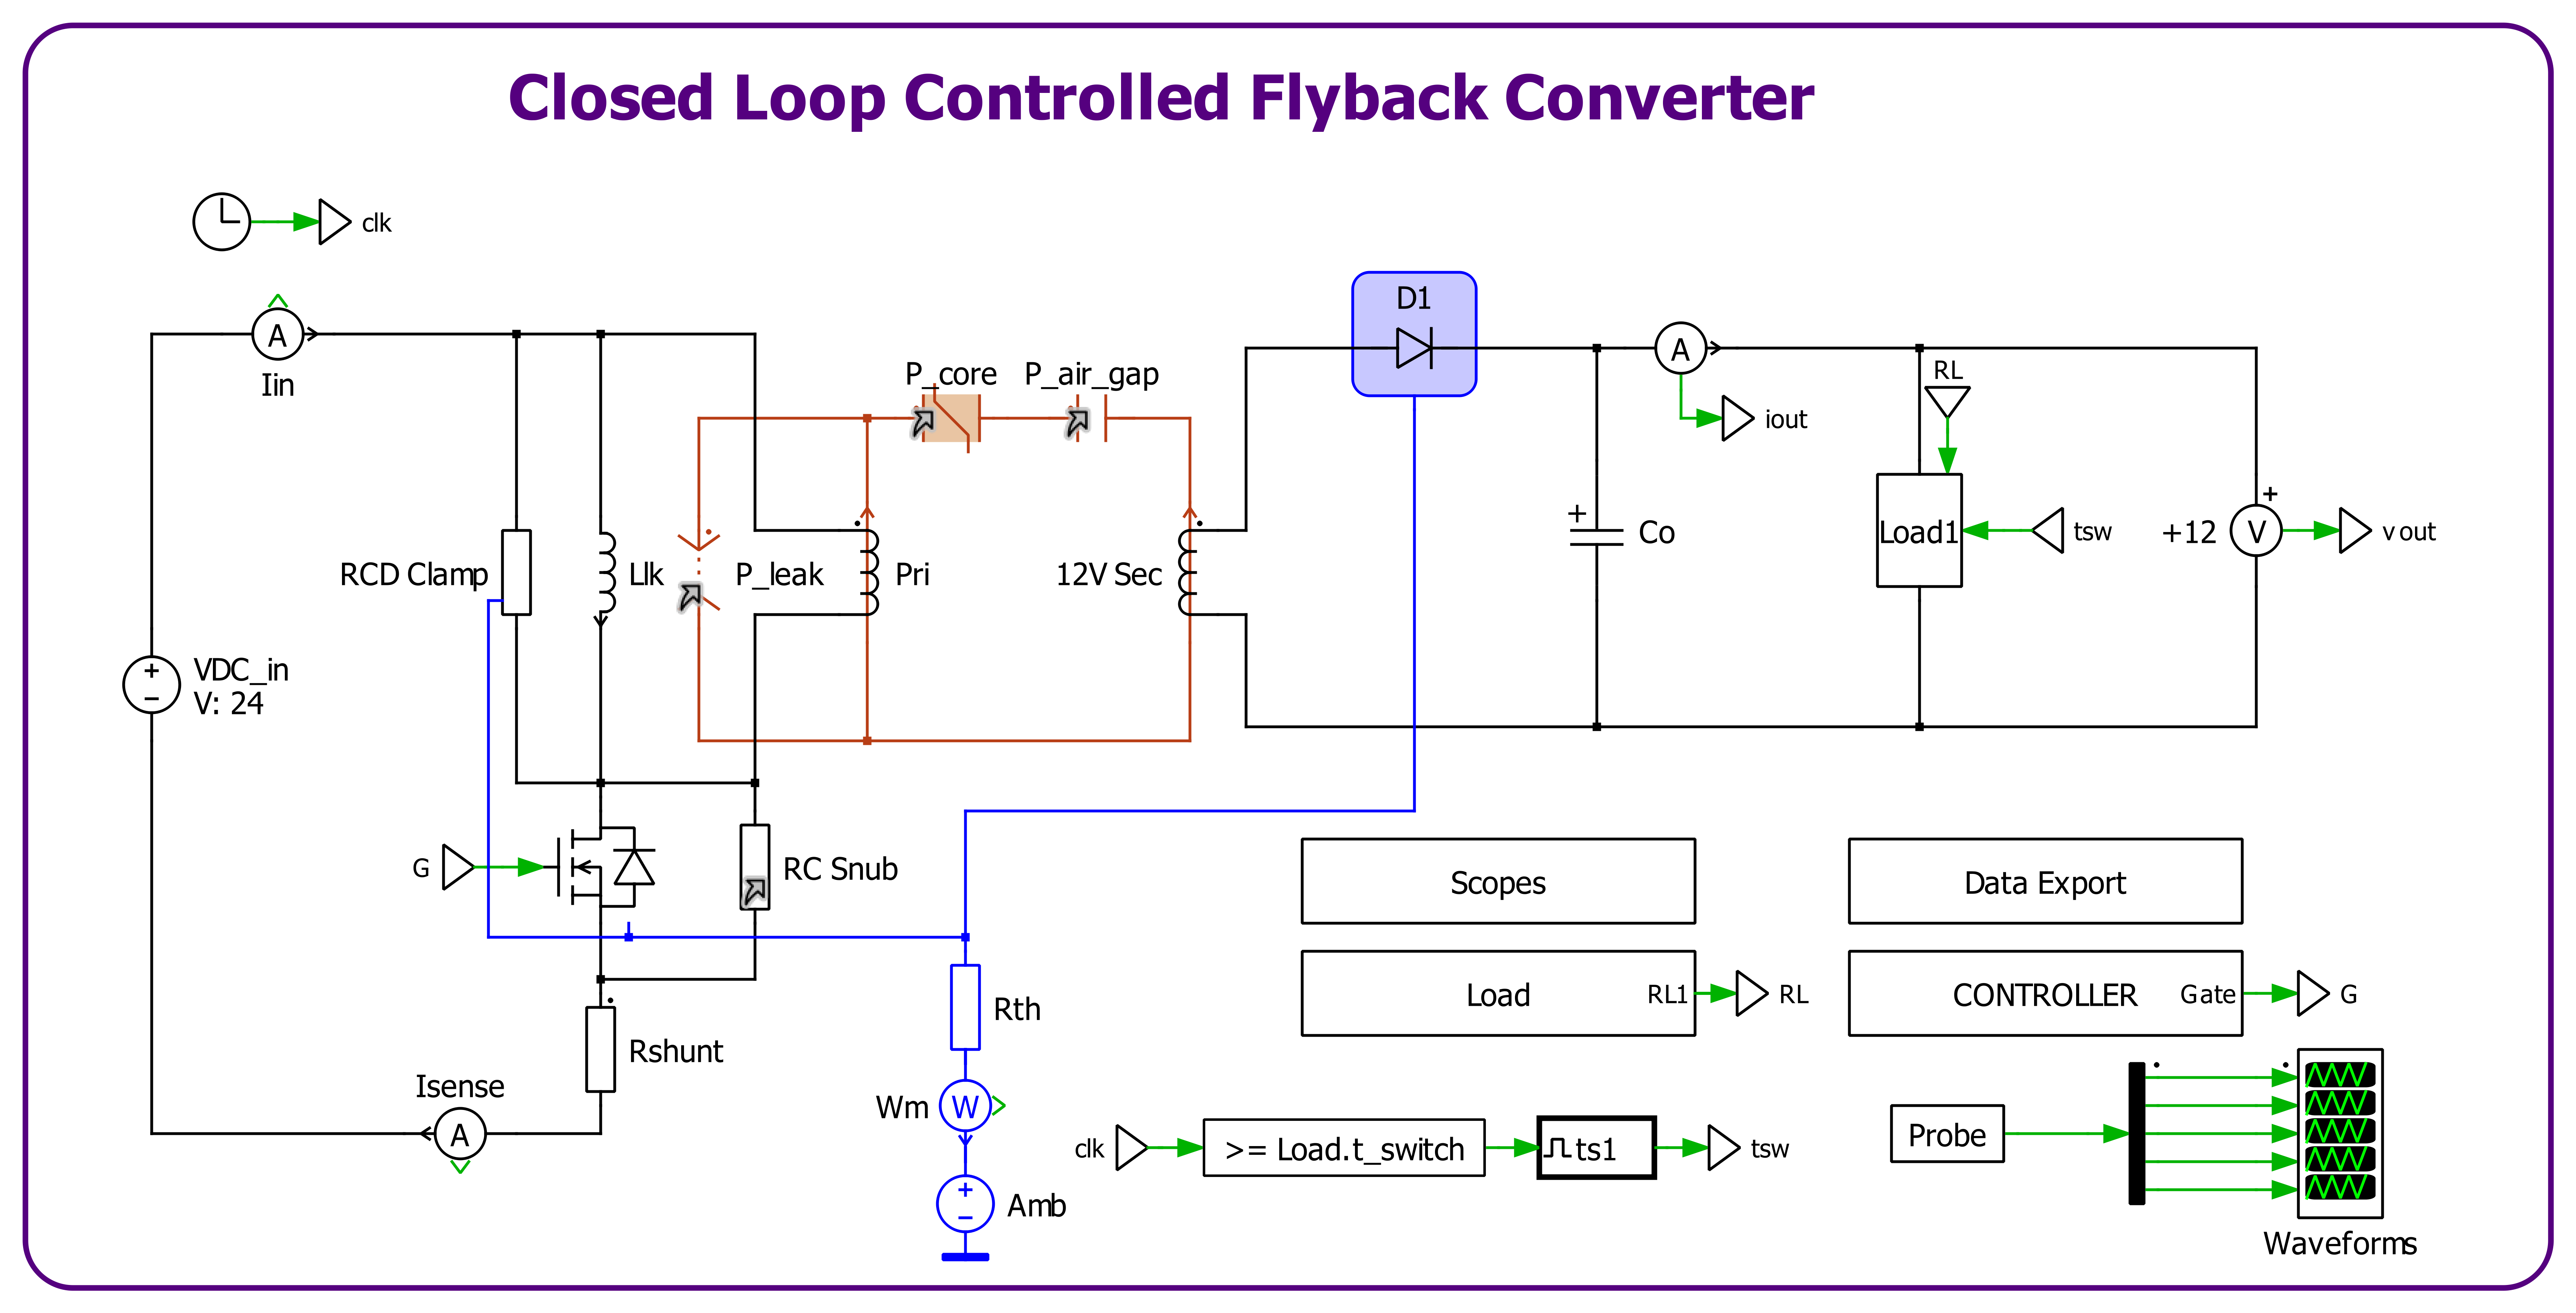
\includegraphics[width=\textwidth]{flyback.jpg}
    \caption{Flyback Converter System Diagram}
    \label{fig:Flyback}
\end{figure}
%-------------------------------------------------------

\section{System Description}
The flyback converter operates by storing energy in a transformer during the switch-on period and releasing it to the output during the switch-off period. This section elaborates on each part of the system.

\subsection{Transformer}
The transformer in a flyback converter serves two primary purposes:
\begin{itemize}
    \item **Energy Storage and Transfer**: During the switch-on period, energy is stored in the transformer's magnetic field. During the switch-off period, this energy is transferred to the output.
    \item **Voltage Transformation and Isolation**: The transformer steps down the input voltage to the required output levels and provides galvanic isolation between the input and the outputs.
\end{itemize}

\subsubsection{Turns Ratio Calculation}
The turns ratio is calculated to meet the output voltage requirements based on the input voltage and the desired duty cycle.

\[
\frac{N_{pri}}{N_{sec1}} = \frac{V_{out1} + V_{f1}}{V_{in} \times D_{max}}
\]

\[
\frac{N_{pri}}{N_{sec2}} = \frac{V_{out2} + V_{f2}}{V_{in} \times D_{max}}
\]

Where:
\begin{itemize}
    \item $N_{pri}$ is the number of turns on the primary winding.
    \item $N_{sec1}$, $N_{sec2}$ are the number of turns on the secondary windings for the 12V and 5V outputs, respectively.
    \item $V_{f1}$, $V_{f2}$ are the forward voltage drops of the diodes.
    \item $D_{max}$ is the maximum duty cycle, which is typically 0.4 to 0.6 for flyback converters.
\end{itemize}

\subsubsection{Primary Inductance}
The primary inductance $L_{pri}$ is crucial for determining the converter’s mode of operation. For continuous conduction mode (CCM), $L_{pri}$ must be sufficiently large.

\[
L_{pri} = \frac{V_{in} \times D_{max} \times (1 - D_{max})}{f_s \times I_{pri, peak}}
\]

Where:
\begin{itemize}
    \item $I_{pri, peak}$ is the peak current through the primary winding.
    \item $f_s$ is the switching frequency.
\end{itemize}

\subsubsection{Core Selection}
The core material and size are selected based on the required inductance and the peak magnetic flux density ($B_{max}$).

\[
B_{max} = \frac{V_{in} \times D_{max}}{N_{pri} \times A_e \times f_s}
\]

Where:
\begin{itemize}
    \item $A_e$ is the effective core area.
\end{itemize}

\subsection{Output Rectification and Filtering}
The output rectification and filtering stages convert the AC voltage from the transformer’s secondary windings into DC voltage and reduce voltage ripple.

\subsubsection{Output Diodes}
The diodes rectify the AC voltage from the transformer into DC. They must be selected based on their peak reverse voltage and average forward current ratings.

\[
V_{R, peak} = V_{in} + V_{out} \times \frac{N_{pri}}{N_{sec}}
\]

\[
I_{avg} = \frac{P_{out}}{V_{out}}
\]

Where:
\begin{itemize}
    \item $V_{R, peak}$ is the peak reverse voltage the diode must withstand.
    \item $I_{avg}$ is the average current the diode must carry.
\end{itemize}

\subsubsection{Output Capacitors}
The capacitors filter the rectified voltage to reduce ripple and provide a stable DC output.

\[
C_{out1} = \frac{I_{out1} \times D_{max}}{f_s \times \Delta V_{out1}}
\]

\[
C_{out2} = \frac{I_{out2} \times D_{max}}{f_s \times \Delta V_{out2}}
\]

Where:
\begin{itemize}
    \item $I_{out1}$ and $I_{out2}$ are the output currents for the 12V and 5V outputs.
    \item $\Delta V_{out1}$ and $\Delta V_{out2}$ are the allowable ripple voltages.
\end{itemize}

\subsection{RC Snubber Circuit}
The RC snubber circuit is used to dampen oscillations caused by the transformer's leakage inductance during the switching transitions.

\subsubsection{Purpose of the RC Snubber}
The RC snubber protects the MOSFET switch from voltage spikes and reduces EMI by damping high-frequency oscillations.

\subsubsection{Snubber Resistor and Capacitor Calculation}
The resistor and capacitor in the snubber circuit are chosen to critically dampen the oscillations.

\[
R_s = \sqrt{\frac{L_{leak}}{C_s}}
\]

\[
C_s = \frac{1}{2 \pi \times f_{ring} \times R_s}
\]

Where:
\begin{itemize}
    \item $L_{leak}$ is the leakage inductance of the transformer.
    \item $f_{ring}$ is the ringing frequency, typically a few MHz.
\end{itemize}

\subsection{RCD Clamp Circuit}
The RCD (Resistor-Capacitor-Diode) clamp circuit limits the peak voltage across the MOSFET by diverting excess energy from the leakage inductance.

\subsubsection{Purpose of the RCD Clamp}
The RCD clamp prevents the MOSFET from being damaged by voltage spikes due to the transformer's leakage inductance.

\subsubsection{Clamp Resistor and Capacitor Calculation}
The clamp resistor dissipates the energy stored in the leakage inductance, and the capacitor stores the energy to limit voltage spikes.

\[
R_{clamp} = \frac{V_{clamp} - V_{in}}{I_{leak}}
\]

\[
C_{clamp} = \frac{\Delta E}{\Delta V_{clamp}^2}
\]

Where:
\begin{itemize}
    \item $V_{clamp}$ is the clamping voltage.
    \item $\Delta E$ is the energy stored in the leakage inductance.
    \item $\Delta V_{clamp}$ is the allowable voltage ripple on the clamp capacitor.
\end{itemize}

\section{Flyback Converter Operation}
The flyback converter operates in two main phases:
\begin{enumerate}
    \item **Switch-On (Energy Storage)**: When the MOSFET switch is on, current flows through the primary winding of the transformer, storing energy in the magnetic field.
    \item **Switch-Off (Energy Transfer)**: When the MOSFET switch is off, the energy stored in the magnetic field is transferred to the secondary windings, where it is rectified and filtered to produce the desired DC outputs.
\end{enumerate}

\section{References}

\begin{enumerate}
    \item R. W. Erickson, \textit{Fundamentals of Power Electronics}, New York: Chapman \& Hall, 1997.
   
\end{enumerate}

\section{Units}

\begin{enumerate}
    \item Farads (\textbf{F}).................: Unit of capacitance.
    \item Amps (\textbf{A})..................: Unit of electric current.
    \item Volts (\textbf{V})...................: Unit of electric potential.
    \item Ohms (\textbf{$\Omega$})............: Unit of electrical resistance.
    \item Henrys (\textbf{H}).................: Unit of inductance.
    \item Watts (\textbf{W}).................: Unit of power.
    \item Hertz (\textbf{Hz}).................: Unit of frequency.
    \item Teslas (\textbf{T})...................: Unit of magnetic flux density.
    \item Webers (\textbf{Wb}).............: Unit of magnetic flux.
    \item Decibels (\textbf{dB}).............: Unit of measurement for the power level of an electrical signal.
\end{enumerate}

%-------------------------------------------------------
\end{document}
%-------------------------------------------------------
